\documentclass[10pt]{article}
\usepackage{float}
\usepackage{listings}
\usepackage[french]{babel}
\usepackage[utf8x]{inputenc}
\usepackage{subcaption}
\usepackage{listings}
\usepackage{wrapfig}
\usepackage{color}
\usepackage{amsmath}
\usepackage{dsfont}
\usepackage{amsfonts}
\usepackage{hyperref}
\usepackage{mathtools}
\usepackage{graphicx}
\usepackage{caption}
\definecolor{dkgreen}{rgb}{0,0.6,0}
\definecolor{gray}{rgb}{0.5,0.5,0.5}
\definecolor{mauve}{rgb}{0.58,0,0.82}
\usepackage[table]{xcolor}
\usepackage{adjustbox}
\usepackage{multirow}
%opening
\definecolor{Gray}{gray}{0.85}




\lstset
{frame=tb,
	language=R,
	aboveskip=3mm,
	belowskip=3mm,
	showstringspaces=false,
	framexleftmargin=5mm,
	columns= fixed,
	numbers = left,
	basicstyle={\small\ttfamily},	
	numberstyle=\tiny\color{gray},
	keywordstyle=\color{blue},
	commentstyle=\color{dkgreen},
	stringstyle=\color{mauve},
	breaklines=true,
	breakatwhitespace=true,
	tabsize=3
}


\title{
	\normalfont \normalsize 
	\textsc{Université de Technologie de Compiègne\\ 
		SY09:Analyse des données et Data-Mining , P17} \\
	[10pt]
	\rule{\linewidth}{0.5pt} \\[6pt] 
	\huge Rendu TP4\\
	\rule{\linewidth}{2pt}  \\[10pt]
}
\author{Zineb Slam, Oumaima Talouka}
\date{\normalsize \today}

\begin{document}
	{\let\newpage\relax\maketitle}	
	
		\begin{abstract}
			Dans de TP4 nous allons étudier 5 techniques de discriminante: l'analyse discriminante linéaire, l'analyse discriminante quadratique, le bayésien naïf, la régression logistique et la régression logistique quadratique. 
		\end{abstract}
	

\section{Programmation}
	\subsection{Analyse discriminante}
	Pour la programmation des 3 modèles de l'analyse discriminante, il nous est demandé de compléter 4 fonctions pré-implémentées.
	Les fonctions \texttt{adq.app}, \texttt{adl.app} et \texttt{nba.app} permettent l'apprentissage des 3 modèles, respectivement l'analyse discriminante quadratique, linéaire et enfin le classifieur bayésien naïf Elles doivent retourner les paramètres des modèles : proportions, moyennes et matrices de covariances des deux classes. Pour cela nous nous sommes appuyés sur les formules suivantes pour chacun des paramètres, dans le cas de l'ADQ: 
	\begin{equation*}
	\widehat{\pi_{k}} = \dfrac{n_{k}}{n}
	\end{equation*}	
	\begin{equation*}
	\widehat{\mu_{k}} = \dfrac{1}{n_{k}}\sum_{i=1}^{n} z_{ik}x{i}
	\end{equation*}
	\begin{equation*}
	\widehat{\Sigma_{k}} = \dfrac{1}{n_{k}}\sum_{i=1}^{n} z_{ik} (x_{i}-\widehat{\mu_{k}})(x_{i}-\widehat{\mu_{k}})^{t}
	\end{equation*} 
	
	En ce qui concerne l'ADL, les proportions et le vecteur des moyennes suivent les mêmes formules. Ce modèle suppose en plus l'hypothèse d'homoscédasticité, donc d'égalité des matrices de variances pour les classes. Celle-ci s'exprime comme suit: 
	\begin{equation*}
	\widehat{\Sigma} = \dfrac{1}{n}\sum_{k=1}^{g} n_{k} \widehat{\Sigma_{k}}
	\end{equation*}	
	Il suffit de sommer les matrices de covariances obtenues par l'ADQ multipliées par les proportions de leurs classes respectives.
	
	Ensuite, pour le modèle du classifieur bayésien naïf, nous supposons l'indépendance des variables conditionnellement à la variable à expliquer Zapp. Donc les formules des proportions et le vecteur des moyennes restent les mêmes, les matrices des covariances se résument aux termes diagonaux, d'ou la multiplication des matrices de covariances obtenues par l'ADQ par la matrice identité. Ce qui donne la formule:  
	 \begin{equation*}
	 \widehat{\Sigma_{k}} = diag(s_{k1}^{2}, ... ,s_{kj}^{2}, ..., s_{kp}^{2} )
	 \end{equation*}
	 
	 Enfin, la 4ème fonction à compléter concerne le calcul des probabilités à posteriori et effectue un classement en fonction de ces probabilités \texttt{ad.val}. Pour le calcul des probabilités à posteriori, nous récupérons les proportions de chaque classe que nous multiplions par la densité à priori de la classe en question calculée grâce à la fonction donnée mvdnorm ( en lui passant la moyenne et la matrice de la covariance de la classe). Puis nous retournons la probabilité à posteriori finale en divisant ce produit par la somme de tous les produits effectués représentant la densité de mélange grâce à \texttt{rowSums} sur R. 
	 
	\subsection{Regression logistique}
	
	Pour la programmation de la régression logistique, il nous est proposé de compléter deux fonctions \texttt{log.app} pour l'apprentissage selon la méthode de Newton-Raphson et \texttt{log.val} pour la validation sur un ensemble de données. La fonction d'apprentissage doit retourner la matrice beta correspondant à l'estimateur du maximum de vraisemblance $\widehat{\beta}$ des paramètres, le nombre \texttt{niter} d'itérations effectuées par l'algorithme de Newton-Raphson, et la valeur $\log L$ de la vraisemblance à l'optimum.
	Pour cela, nous utilisons les formules suivantes respectivement aux paramètres retournés par la fonction à compléter et de manière itérative la formule (\ref{eq:newton-raphson}) à l'aide du calcul des formules détaillées de la matrice hessienne et le gradient de la log-vraissemblance calculés en $w^{(q)}$  jusqu'à convergence (nous rappelons qu'un vecteur de poids initial $w^{(0)}$ est choisi avant le début de la séquence) : 
	
	\begin{equation} \label{eq:newton-raphson}
	w^{(q+1)} = w^{(q)}-H^{-1}_{(q)}*\dfrac{\partial \log L}{\partial w}(w^{(q)})
	\end{equation}
	\begin{equation*}
	H_{(q)} = -X^{T}W_{(q)}X
	\end{equation*}
	\begin{equation*}
	\dfrac{\partial \log L}{\partial w}(w^{(q)}) = X^{T}(t-p^{(q)})
	\end{equation*}
	
	Nous arrêtons la séquence d'itérations lorsque la nouvelle estimation $w^{(q+1)}$ et $w^{(q)}$ est inférieure au seuil fixé $\epsilon$ comme variable d'entrée de la fonction \texttt{epsi}. 
	
	Nous avons aussi complété la fonction \texttt{post.prob} qui calcule les probabilités à posteriori en fonction du paramètre beta retourné par la fonction d'apprentissage. Nous utilisons pour cela les formules suivantes : 
	
	\begin{equation*}
	P(w_{1}|x) = p(x,w) = \dfrac{\exp(w^{t}x)}{1+\exp(w^{t}x)}
	\end{equation*}
	\begin{equation*}
	P(w_{2}|x) = 1-p(x,w)
	\end{equation*}
	
	Cette dernière nous aida dans l'implémentation de la fonction de validation \texttt{log.val}. Nous l'utilisons pour récupérer les fonctions de probabilités et nous utilisons \texttt{cbind} de R afin de retourner la matrice des probabilités à posteriori des deux classes dans le cas binaire de la régression logistique correspondant à \texttt{prob} et \texttt{1-prob} et le vecteur des classements associés.
	\\
	\\
	\textbf{Régression logistique quadratique}
	 Pour pouvoir appliquer ce modèle, il faudra adapter l'ensemble des données d'entrée \texttt{Xapp} à la méthode décrite dans l'énoncé. Pour cela nous procédons comme suit: 
	\begin{lstlisting}
	Xapp = as.matrix(Xapp)
	Xapp = cbind(Xapp, Xapp[,1]*Xapp[,2], Xapp[,1]*Xapp[,1], Xapp[,2]*Xapp[,2])
	\end{lstlisting}
	
\section{Application}
\subsection{Test sur données simulées}
Pour séparer nos données en ensemble d'apprentissage et de test nous faisons de la sorte:
\begin{lstlisting}
train   = sample(1:n, round(2*n/3)) 
Xapp    = X[train, ]
zapp    = z[train]
Xtst  = X[-train, ]
ztst  = z[-train]
\end{lstlisting}
\subsubsection{Synth1-1000}
Nous avons représenté les résultats de calcul de l'erreur de test dans les données Synth1-1000. 
\begin{center}
	\begin{tabular}{|c | c | c| c| c| c|}
		\hline
		LDA & QDA & Naive Bayes & Log Reg & Quad Log Reg & Tree\\
		\hline	
		4.62\% & 3.60\% & 4.17\% & 3.75\% & 3.63\% & 4.88\%
	\end{tabular}
\end{center}
Nous retrouvons les taux d'erreur les plus bas pour l'ADQ et les régressions logistiques. Nous en déduisons que les données suivent bien des distributions normales et qu'il est fort probable que les classes ont des matrices de covariances différentes (l'hypothèse d'homoscédasticité n'est pas vérifiée). 

Les graphes sont représentés ci-dessous avec les frontières de décisions.

\begin{minipage}{.5\textwidth}
	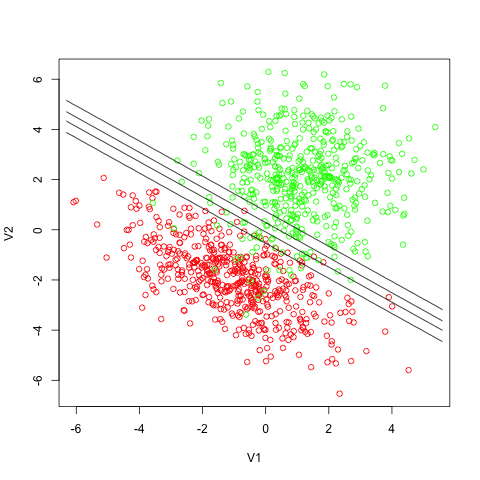
\includegraphics[width=45mm]{Figures/synth1_lda.png}
\end{minipage}%
\hspace{0.02\linewidth}
\begin{minipage}{.5\textwidth}
	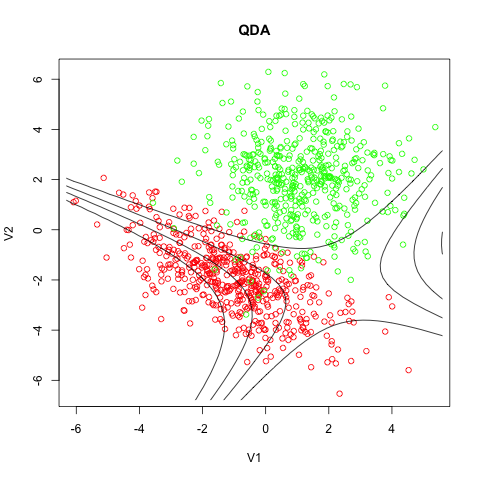
\includegraphics[width=45mm]{Figures/synth1_qda.png}
\end{minipage}

\begin{center}
	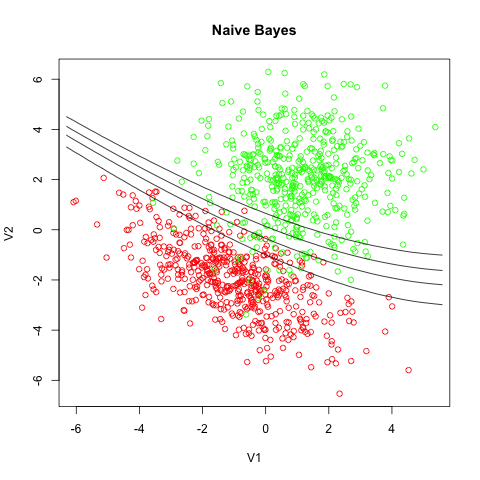
\includegraphics[width=45mm]{Figures/synth1_nb.png}
\end{center}
\begin{minipage}{.5\textwidth}
	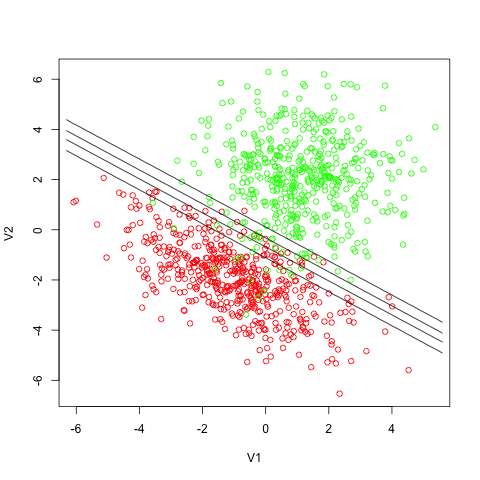
\includegraphics[width=45mm]{Figures/synth1_logreg.png}
\end{minipage}%
\hspace{0.02\linewidth}
\begin{minipage}{.5\textwidth}
	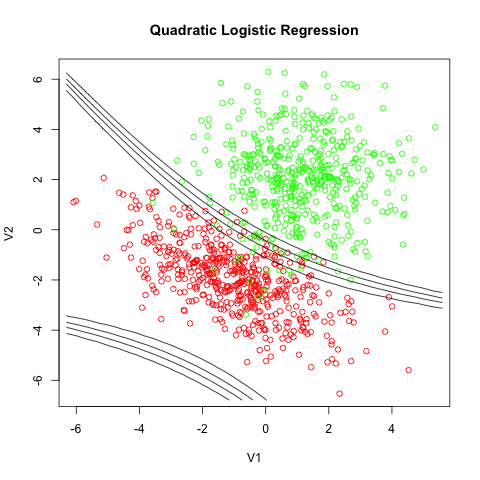
\includegraphics[width=45mm]{Figures/synth1_logregquad.png}
\end{minipage}

\subsubsection{Synth2-1000}
Dans ce qui suit nous avons représenté les résultats de calcul de l'erreur de test dans les données Synth2-1000. 
Nous avons représenté les résultats de calcul de l'erreur de test dans les données Synth1-1000. 
\begin{center}
	\begin{tabular}{|c | c | c| c| c| c|}
		\hline
		LDA & QDA & Naive Bayes & Log Reg & Quad Log Reg & Tree\\
		\hline	
		8.05\% & 6.30\% & 6.30\% & 7.10\% & 6.38\% & 7.98\%
	\end{tabular}
\end{center}
Les graphes sont représentés ci-dessous avec les frontières de décisions et les erreurs pour chaque classifieur.

\begin{minipage}{.5\textwidth}
	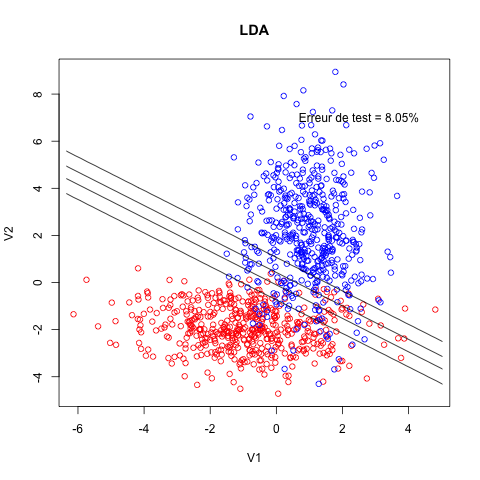
\includegraphics[width=45mm]{Figures/synth2_lda.png}
\end{minipage}%
\hspace{0.02\linewidth}
\begin{minipage}{.5\textwidth}
	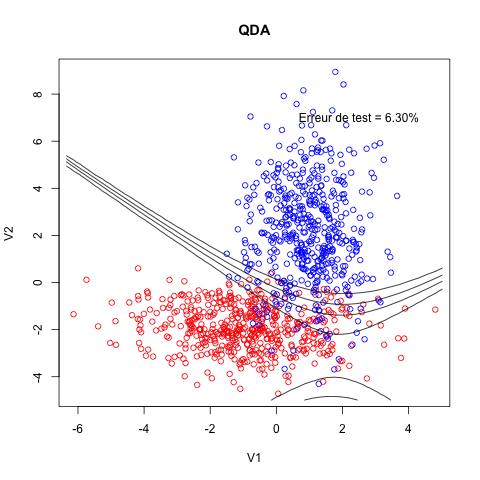
\includegraphics[width=45mm]{Figures/synth2_qda.png}
\end{minipage}

\begin{center}
	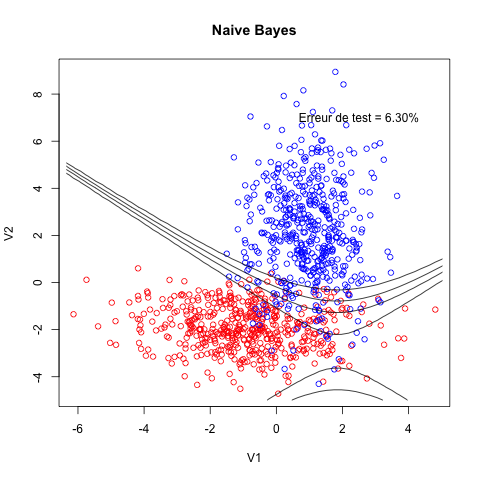
\includegraphics[width=45mm]{Figures/synth2_nb.png}
\end{center}
\begin{minipage}{.5\textwidth}
	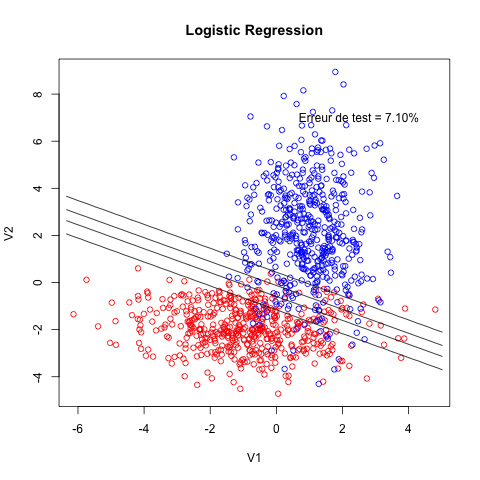
\includegraphics[width=45mm]{Figures/synth2_logreg.png}
\end{minipage}%
\hspace{0.02\linewidth}
\begin{minipage}{.5\textwidth}
	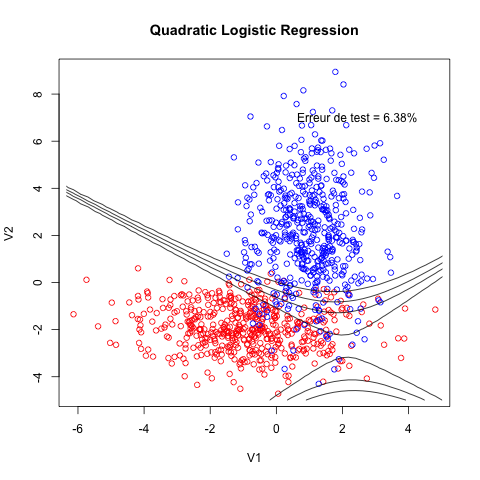
\includegraphics[width=45mm]{Figures/synth2_logregquad.png}
\end{minipage}


On remarque que l'erreur de test est inférieure a  9\% pour tous les classifieurs. Selon la représentation des points on remarque que les classes ont à peu près la même distribution et on n'a qu'une dizaine de points qui sont confondus entre les 2 classes. Par conséquent les classes peuvent être  linéairement séparées, ceci est illustré par l'erreur de test puisqu'on voit que la régression quadratique n'apporte qu'une légère amélioration de l'ordre de 1\%.
Néanmoins il faut remarquer que le classifieur Bayésien Naïf performe aussi bien que les régressions quadratiques. Ceci était prévisible vu que nos classes sont orientées vers les axes du plan. Ainsi il est plus intéressant dans ce cas d'utiliser le classifieur Bayésien Naïf vu qu'on n'estime moins de parametres qu'avec  la régression quadratique ou même la logistique quadratique.


\subsubsection{Synth3-1000}
Nous nous intéressons à présent aux données de Synth3-1000 avec 1000 individus.

Nous avons représenté les résultats de calcul de l'erreur de test dans les données Synth1-1000. 
\begin{center}
	\begin{tabular}{|c | c | c| c| c| c|}
		\hline
		LDA & QDA & Naive Bayes & Log Reg & Quad Log Reg & Tree\\
		\hline	
		4.11\% & 4.7\% & 4.89\% & 4.14\% & 4.16\% &6.55\%
	\end{tabular}
\end{center}

\begin{minipage}{.5\textwidth}
	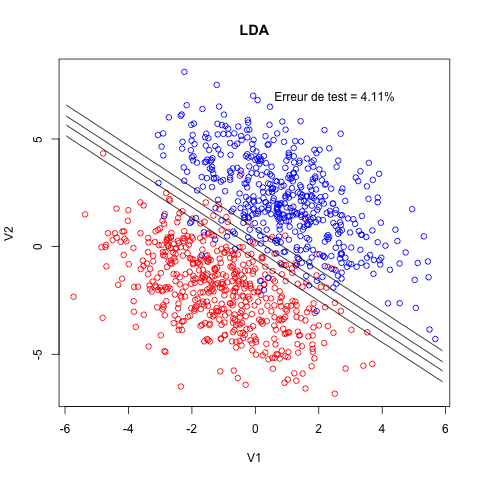
\includegraphics[width=45mm]{Figures/synth3_lda.png}
\end{minipage}%
\hspace{0.02\linewidth}
\begin{minipage}{.5\textwidth}
	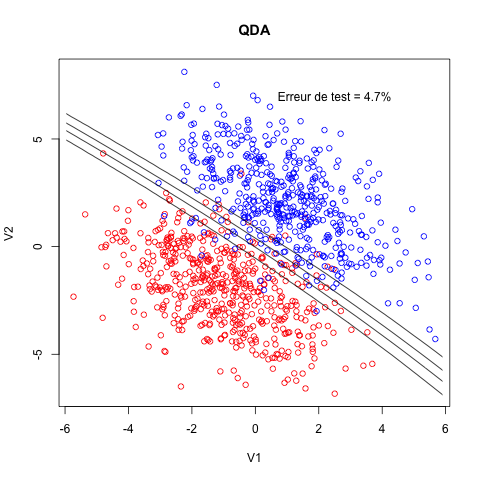
\includegraphics[width=45mm]{Figures/synth3_qda.png}
\end{minipage}

\begin{center}
	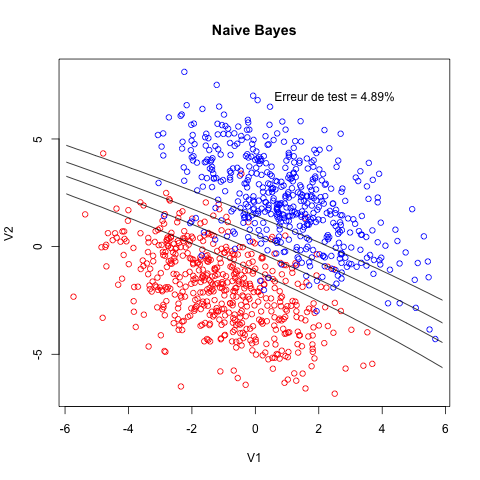
\includegraphics[width=45mm]{Figures/synth3_nb.png}
\end{center}
\begin{minipage}{.5\textwidth}
	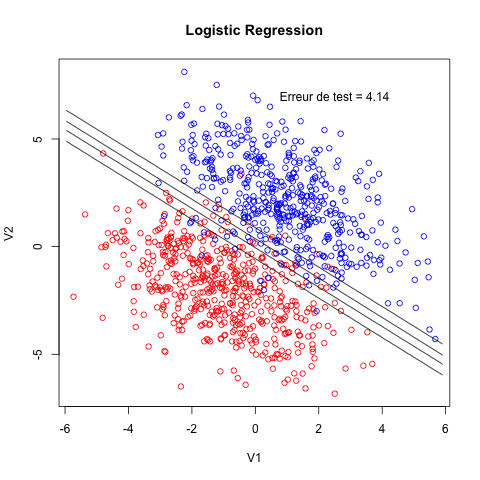
\includegraphics[width=45mm]{Figures/synth3_logreg.png}
\end{minipage}%
\hspace{0.02\linewidth}
\begin{minipage}{.5\textwidth}
	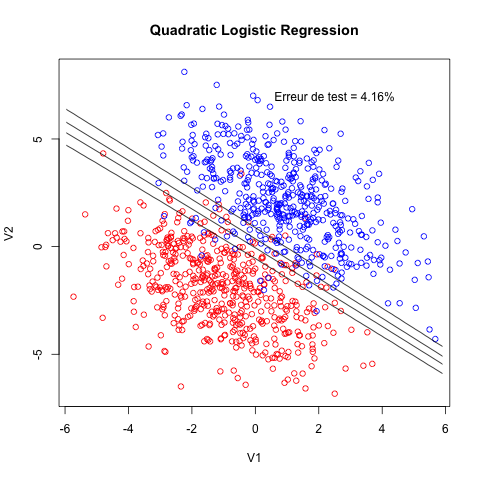
\includegraphics[width=45mm]{Figures/synth3_logregquad.png}
\end{minipage}

On remarque en représentant les données que les classes ont les mêmes orientations et distributions, elles peuvent être linéairement séparées.  Il est donc normal de voir que les erreurs de test du LDA sont faibles et que celles ci sont approximativement égales à celles du QDA. 


\subsection{Test sur données réelles}
\subsection{Pima}
Ce jeu de données concerne des individus d'une population d’amérindiens et la prédiction du diabète selon les caractéristiques présentées. 

\begin{center}
	\begin{tabular}{|c | c | c| c| c| c|}
		\hline
		LDA & QDA & Naive Bayes & Log Reg & Quad Log Reg & Tree\\
		\hline	
		22.31\% & 24.20\% & 24.02\% & 22.18\% & 23.65\% & 25.72\%
	\end{tabular}
\end{center}

Nous remarquons que les taux d'erreurs sont considérablement élevés pour ce dataset. Ils tournent autour du 24\%, ce qui fait 20\% plus élevé que les données simulées analysées précédemment. Nous nous rappelons que les plots des données quantitatives de Pima lors de leur analyse au TP1 ne nous permettaient pas de distinguer les classes présentant le critère de présence du diabète ou pas. Il fut difficile de déterminer si une des variables explicatives permettait de décider de leur différenciation, nous pouvons le voir sur la figure (\ref{fig:plotPima}). 
\begin{figure}[H]
	\centering
	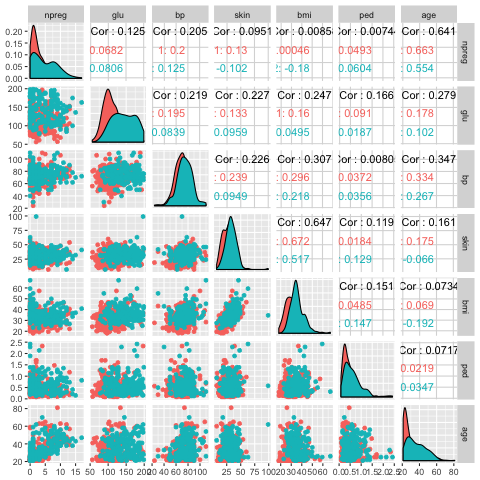
\includegraphics[width=9cm]{Figures/plot_Pimaquant.png}%
	\caption{Plots des données Pima}%
	\label{fig:plotPima}
\end{figure}

\subsection{Breast Cancer}
\subsubsection{Description des données}
Avant de se lancer dans l'analyse de données, nous allons essayer de décrire ces données pour mieux analyser les résultats obtenus. Breast Cancer Winsconsin compte 683 individus et 9 variables quantitatives explicatives.
\subsubsection{Analyse discriminantes et régression logistique}
Le tableau ci-dessous montrent les résultats obtenus avec les différentes méthodes d'analyses discriminantes et de régression logistique.
\begin{center}
	\begin{tabular}{|c | c | c| c| }
		\hline
	LDA & QDA & Naive Bayes & Log Reg \\
	\hline	
	4.57\% & 5.03\% & 3.98\% & 4.02\%
	\end{tabular}
\end{center}

Contrairement aux résultats obtenus dans les données de \textit{Synth} on remarque ici que les performances des classifieurs diffèrent. En effet le classifieur Bayésien Naïf et la régression logistique sont ceux qui classent au mieux nos données suivis par la méthode d'analyse discriminante linéaire et quadratique. 
La méthode la plus performante ici est le classifieur Bayésien Naïf. En effet si on s'intéresse à la matrice de variance, on remarque que les valeurs dans la diagonale sont les plus grandes. La matrice est donc quasi-diagonale. Ce qui vérifie l'hypothèse d'indépendance des données du classifieur Bayésien Naïf. \\
La méthode d'analyse linéaire n'est pas aussi performante car si on observe les matrices de variances de chaque classe, on remarque que l'hypothèse d'homoscédasticité n'est pas vérifiée.

\subsubsection{Conclusion}
On remarque que dans les 3 cas, la régression logistique fournit le pourcentage d'erreur le plus faible. Néanmoins cette méthode est trop couteuse quant au nombre de paramètres à estimer. Remarquons qu'appliquer la méthode de régression logistique quadratique aurait été trop couteux dans ce cas ou on a 8 variables d'une part. 

\subsubsection{Arbres de décisions}
Pour obtenir l'arbre de décision de l'ensemble d'apprentissage nous utilisons la fonction \textit{tree} du \textit{package tree}. Nous fixons les paramètres\\  \textit{control=tree.control(nobs=dim(Dapp)[1],mindev = 0.0001)}  comme demandé dans ce TP. \textit{nobs} est le nombre d'observations des données d'apprentissage , \textit{mindev} est la déviance entre les nœuds. Si mindev=0 il essaye de placer parfaitement les données. La fixation de ces paramètres influence directement la taille (le nombre de nœuds) de l'arbre.\\
\begin{minipage}{.5\textwidth}
	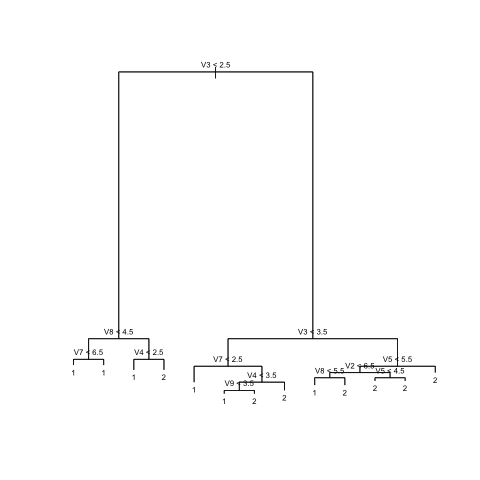
\includegraphics[width=50mm]{Figures/bcw_apptree.png}
\end{minipage}%
\hspace{0.001\linewidth}
\begin{minipage}{.5\textwidth}
	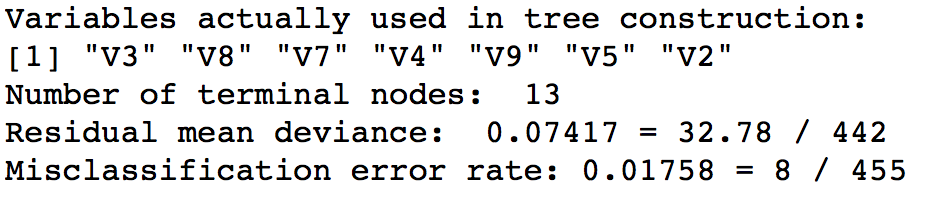
\includegraphics[width=65mm]{Figures/bcw_apptree_summary.png}
\end{minipage}

Ainsi sur l'ensemble d'apprentissage on a une erreur de mal classement de 1.76\%. On remarque ici V3, V8, V7, V8, V9, V5 et V2. La  complexité d'un arbre est évaluée avec le nombre de feuilles qu'il a puisque se sont les différentes classes. Ainsi la fonction \textbf{tree} nous retourne un arbre avec 13 nœuds et donc 13 partitions.\\
Nous allons à présent utiliser la méthode de cross validation pour trouver la hauteur optimale de l'arbre. On utilise la fonction R \textbf{tree.cv} avec k=10 pour faire une \textit{10-fold cross validation}, qui consiste à diviser l'ensemble d'apprentissage en 10 ensembles et utiliser un à chaque fois comme ensemble de validation.  Les résultats sont représentés ci-dessous sous forme du graphe de l'évolution du nombre d'individus mal classés en fonction de la taille de l'arbre qui est égale au nombre de feuilles.

\begin{minipage}{.4\textwidth}
	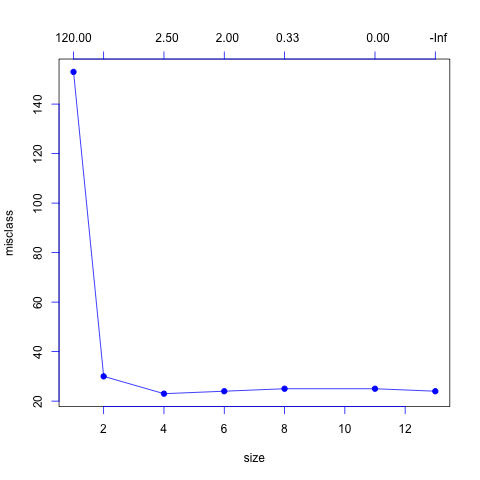
\includegraphics[width=45mm]{Figures/bcw_cvplot.png}
		\captionof{figure}{Graphe de l'evolution des individus mal-classes en fonction du nombre de feuilles}
\end{minipage}%
\hspace{0.01\linewidth}
\begin{minipage}{.65\textwidth}
 \begin{lstlisting}
min= which(bcw.cv$dev==min(bcw.cv$dev))
best.size= bcw.cv$size[min]
 \end{lstlisting}
\end{minipage}

On récupère donc la taille de l'arbre qui minimise l'erreur (le nombre d'individus mal classes) qui est 4. Ensuite on utilise la fonction\textbf{prune.misclass} permet d’élaguer l’arbre en mettant 4 comme taille de l'arbre. Grâce à la fonction \textbf{predict} on obtient en sortie le vecteur de prédiction de classes. La matrice ci-dessous est la matrice de confusion des vrais classements et des prédictions.
\begin{minipage}{.5\textwidth}
	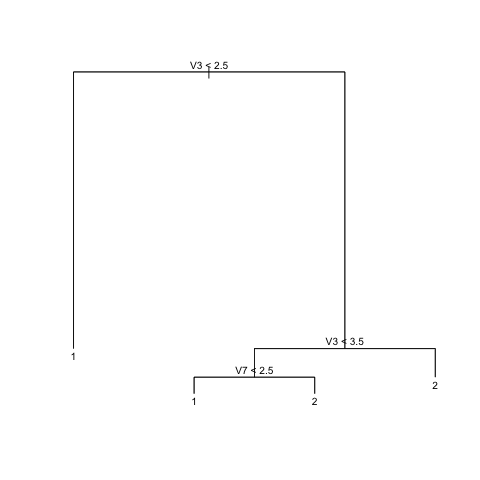
\includegraphics[width=45mm]{Figures/bcw_prunedtree.png}
\end{minipage}%
\hspace{0.00\linewidth}
\begin{minipage}{.4\textwidth}
\begin{tabular}{c  c c}
  & 1  &  2 \\
1 & 135 &   7 \\
2 &  6&  80
\end{tabular}
\end{minipage}

Nous utilisons ensuite les instructions pour calculer l'erreur de test:
\begin{lstlisting}
tree.pred = predict(bcw.cv.pruned, Xtst, type = "class")
res = with(Xtst, table(tree.pred, ztst))
error.test = res[1,2] + res[2,1] / nrow(Xtst)
print(paste("Test Error  ",error.test))
\end{lstlisting}

Nous obtenons 6.03\% comme erreur de test.

\section{Spams challenge}

On considère dans ce challenge un dataset traitant de la détection de spams à partir d'indicateurs calculés sur des messages électroniques 

Ce jeu de données comprend 58 variables explicatives et une variable à expliquer. Nous remarquons que pour certaines variables il y a un nombre significativement grand d'individus portant des informations nulles. 
L'existence de matrice creuse peut induire à des matrices de covariances non inversibles. 
Lorsque nous avons de tels grands jeux de données, la première chose à faire est de centrer et réduire notre matrice d'apprentissage puis d'appliquer \textbf{cette même transformation} à notre ensemble de test.\\ 

Nous avons commencé notre discrimination par une méthode simple qui est le K-PPV afin d'obtenir une idée générale de l'erreur. Nous avons utilisé la méthode de 5-fold cross validation pour déterminer le meilleur k. L'erreur obtenue est très supérieure avec le K-NN.\\

La méthode de centrage nous a permis d'avoir des résultats concrets pour la régression logistique et le classifieur bayésien naïf Cependant, nous n'avons pas pu obtenir de résultats pour les analyses discriminantes quadratique et linéaire. Nous pensons que cela est du é la matrice hessienne qui est non semi-positives. Nous pensons aussi que l'instabilité numérique a une influence sur les calculs effectués sur ce dataset.\\

Par ailleurs, nous avons eu recours au modèle de l'arbre de décision \texttt{tree} et \texttt{randomForest}. Avec un choix judicieux de la taille de l'arbre (taille = 7), nous avons pu avoir un taux d'erreur faible avec ce modèle. La foret aléatoire (Random Forest) est une méthode puissante car elle sélectionne aléatoirement un sous ensemble de variables en introduisant la diversité dans l'arbre. Ceci n'est pas forcément un critère d'optimalité mais permet de mieux apprendre le modèle.

Le tableau ci-dessous montrent les résultats obtenus avec les différentes méthodes:
\begin{center}
	\begin{tabular}{c |c | c | c| c| c| c|}
		\hline
		KNN & LDA & QDA & Naive Bayes & Log Reg & Tree & Random Forest\\
		\hline	
		40.04\% & NA &  NA &17.27\% & 6.39\% &  0.065\%& 1.24\%
	\end{tabular}
\end{center}

Nous pensons qu'une utilisation de l'analyse factoriel discriminante (AFD) aurait donné de meilleures résultats que l'ACP. En effet avec l'AFD on exprime la matrice de variance comme $\Sigma = W + B$ avec B la matrice de variance inter-classes (between classes) et W la matrice de variance intra-classes (Within-classes), puis on essaye de maximiser B. Par conséquent l'AFD vise à séparer le mieux possible les classes en maximisant la variance inter-classes (Between Classes). Nous avons vu que cette méthode peut être implémentée par la fonction \textit{lda} sur R mais nous n'avons malheureusement pas pu la mettre en place par faute de temps. 
\end{document}